\documentclass{article}[18pt]
\usepackage{../../../../format}
\lhead{Software Methodolgies - Image Processing}


\begin{document}
\begin{center}
\underline{\huge Point transforms - arithmetic \& logical operations}
\end{center}
\section{Matrices}
If our image is a matrix then can process (transform) an image by manipulating the corresponding matrix\\
We can process (transform) images by manipulating the corresponding matrices
\begin{center}
	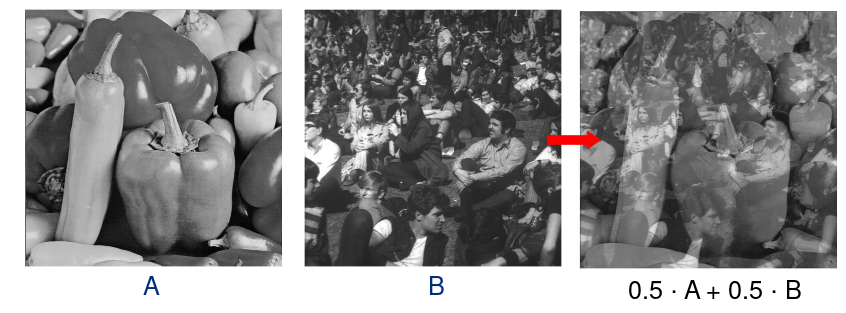
\includegraphics[scale=0.7]{matrices}
\end{center}
\section{Transformation aims}
Four categories:
\begin{itemize}
	\item \textbf{Remove image degradations} introduced during capture
	\item \textbf{Improve image appearance} for viewing or further processing (i.e. image enhancement)
	\item \textbf{Identify image features} for recognition of scene objects
	\item \textbf{Transform image to alternative representation} for efficient processing 
\end{itemize}
\section{Types of image transforms}
An image transform processing $I_{input}$ to $I_{output}$ may be:
\begin{itemize}
	\item A point transform involving only a single pixel at a time
	\item A local transform involving the local image neighbourhood (pixel+those immediately "next to it" - later in course)
	\item A global transform involving the whole image (later in course)
\end{itemize}
\section{Basic point transforms}
Point transforms map individual points in the input image to individual points in the output image\\
\\
Performed as an operation, denoted o, between to images, $I_A$ and $I_B$, or between an image and a constant value C:
$$I_o=I_A\circ I_B$$
$$I_o=I_A\circ C$$
Pixel location (i,j) in the output image is computed as follows
$$I_o(i,j) = I_A(i,j) \circ I_B(i,j)$$
$$I_o(i,j)=I_A(i,j)\circ C$$
Apply transform iteratively over the image indices for $(i,j)=\{0...w-1,0..h-1\}$\\
w= image width\\
h= image height
\section{Arithmetic operations}
\subsection{Addition}
Operation: adding a value to each image pixel\\
Application brightness adjustment: adding a positive constant value to each pixel increases brightness\\
\\
Application blending: adding images together produces a composite image of both inputs
\begin{center}
	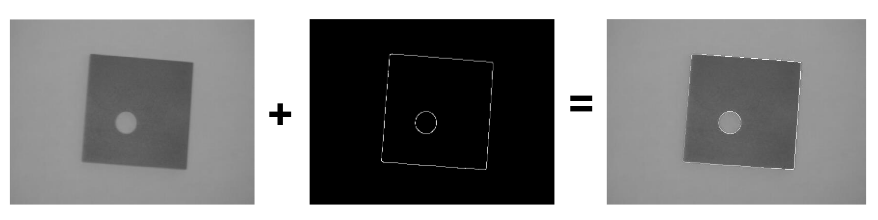
\includegraphics[scale=0.7]{addition}
\end{center}
In both cases watch for integer overflow. The result of the addition can be out of range
\subsection{Subtraction}
Operation: subtracting a value to each image pixel\\
Application brightness adjustment: as per addition\\
\\
Image subtraction can be used to see where things have moved in a scene. However it is subjects to high levels of noise.
\subsection{Division}
Operation: dividing each image pixel by a value\\
Application brightness adjustment: uniformly scale image intensities e.g. reduce to 25\% of the original by dividing by 4\\
Application image differencing: dividing an image by another\\
This is less efficient than subtraction
\begin{center}
	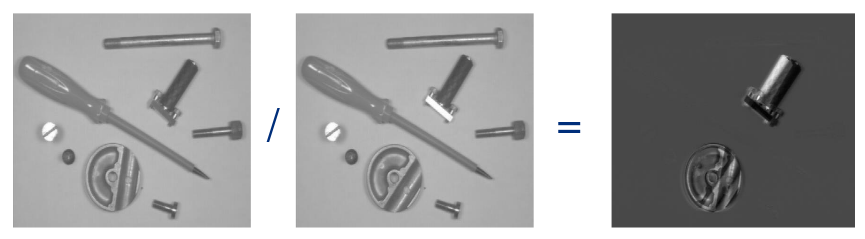
\includegraphics[scale=0.7]{division}
\end{center}
\subsection{Multiplication}
Operation: multiplying each image pixel by a value (equivalent to division by the inverse of that value)\\
Application brightness adjustment: pixel value scaling as per division 
\section{Application: image blending}
Image blending is an application of image arithmetic operations producing ghosting or overlay effects between different images\\
\\
N images $I_1,I_2,...,I_n$ can be blended in equal proportions
\[
I_{\text {output}}=\sum_{i} \frac{1}{N} I_{i}
\]
Alternatively, different weights can be used between images to enhance/suppress the features of different images in the final result
\begin{center}
	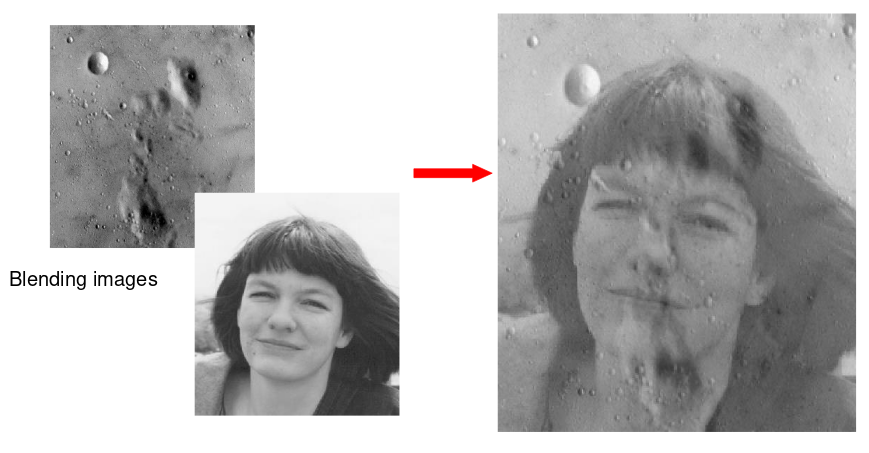
\includegraphics[scale=0.7]{image_blending}
\end{center}
\section{Bit planes}
Intuitively, logical (bit-wise) operations can be thought of as applied on bit planes
\begin{center}
	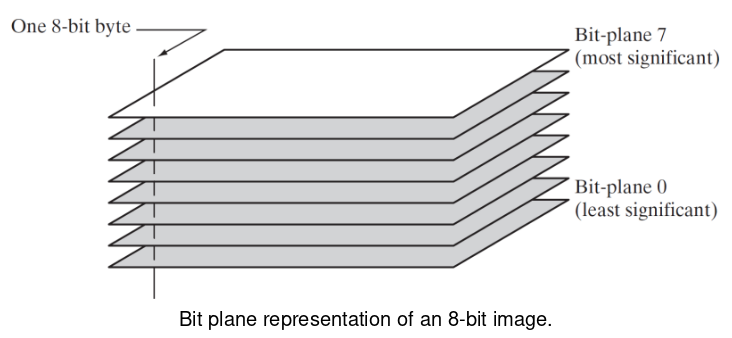
\includegraphics[scale=0.7]{bit_planes}
\end{center}
\begin{itemize}
	\item The most significant bit contains most of the information in the image, and so image processing could just be done on that
	\item Bit planes are used so that image processing can have a less complex image to deal with, and so is faster
\end{itemize}
\section{Logical operations}
\subsection{NOT (inverse)}
Operation: logical NOT to invert the image\\
\\
For binary images, white pixels become black and vice versa\\
\\
For 8-bit greyscale images (or 8-bit colour channels)
$$I_{output}=255-I_{input}$$
Image inversion is an invertible operation\\
\\
On colour (and greyscale) images it produces the photographic negative effect
\subsection{AND}
Can be used for:
\begin{itemize}
	\item Detecting differences or overlap between images - Not(A) and Not(B)
	\item Highlighting appropriate regions with a mask - All black with white round selection
	\item Slicing bit planes through an image  - And with powers of 2
	\item Superimpose images
\end{itemize}
\subsection{OR}
An OR operation can be replaced by AND and NOT operations via:
\begin{center}
	A OR B = =NOT(NOT(A) AND NOT(B))
\end{center}
Can do basic image overlays but no control on weighing available\\
\\
Quality of OR based overlay is contrast dependant\\
Here, controlled blending is better
\subsection{XOR}
XOR is a very useful tool in efficiently detecting image differences as it highlights only where change occur
% Got up to here in the lecture
\section{Colour to Greyscale}
This is a non invertible, lossy transform, information is destroyed. \\
\\
A simple way to do the conversion is to take a weighted sub of the R,G,B values:
\begin{itemize}
	\item Input RGB colour image, $I_c$
	\item Output Grayscale image, $I_g$
\end{itemize}
$$I_g=\alpha I_c (R) + \beta I_c (G) + \gamma I_c(B)$$
The coefficients $(\alpha, \beta, \gamma)$ are usually taken in proportion to the human vision sensitivity to the R,G,B colour channels\\
\\
One commonly used weighting for the conversion is (NTSC television standard). $\alpha=0.2989, \beta = 0.5870$ and $\gamma=0.1140$
\section{Computational Complexity}
Square $n\times n$ images have $n^2$ pixels\\
\\
Computational cost of a point transform applied to the whole image $\mathcal{O}(n^2)$\\
\\
Quadratic runtime means that the total number of CPU operations increases rapidly as the image size increases\\
\\
Solutions:
\begin{itemize}
	\item Parallel processing (traditional)
	\item Image pyramid approaches: down size image, do the processing, then up-size again
\end{itemize}


\end{document}